\documentclass[11pt,letterpaper]{article}
\usepackage[lmargin=1in,rmargin=1in,tmargin=1in,bmargin=1in]{geometry}

% -------------------
% Packages
% -------------------
\usepackage{
	amsmath,			% Math Environments
	amssymb,			% Extended Symbols
	enumerate,		    % Enumerate Environments
	graphicx,			% Include Images
	lastpage,			% Reference Lastpage
	multicol,			% Use Multi-columns
	multirow,			% Use Multi-rows
	tikz,
	wrapfig,
	xcolor,
	float,
	enumitem	
}
\usetikzlibrary{intersections}

\setlength{\parskip}{\baselineskip}%
\setlength{\parindent}{0pt}%

\newlist{problemslist}{enumerate}{1}
\setlist[problemslist]{
	label = \textbf{Problem \arabic*.}, 
	wide
}

\title{MATH4.1 Trigonometry}
\author{T Yeung}

\usepackage[T1]{fontenc}
\usepackage{charter}

\newcommand{\prob}{\noindent\textbf{Problem. }}
\newcounter{problem}
\newcommand{\problem}{
	\stepcounter{problem}%
	\noindent \textbf{Problem \theproblem. }%
}
\newcommand{\pointproblem}[1]{
	\stepcounter{problem}%
	\noindent \textbf{Problem \theproblem.} (#1 points)\,%
}
\newcommand{\pspace}{\par\vspace{\baselineskip}}
\newcommand{\ds}{\displaystyle}


\usepackage{fancyhdr}

\fancypagestyle{pages}{
	%Headers
	\fancyhead[L]{}
	\fancyhead[C]{}
	\fancyhead[R]{}
	\renewcommand{\headrulewidth}{0pt}
	%Footers
	\fancyfoot[L]{}
	\fancyfoot[C]{}
	\fancyfoot[R]{}
	\renewcommand{\footrulewidth}{0.0pt}
}
\headheight=0pt
\footskip=14pt

\pagestyle{pages}


% -------------------
% Content
% -------------------
\begin{document}
\maketitle
\section{Motive}

\begin{wrapfigure}{r}{0.35\textwidth}
	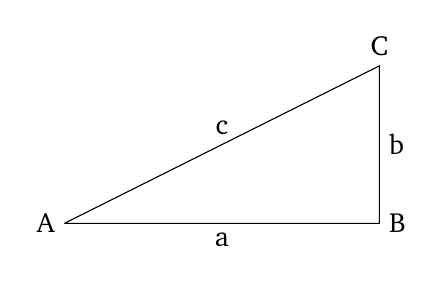
\begin{tikzpicture}
		\coordinate (a) at (0,0);
		\coordinate (b) at (4,0);
		\coordinate (c) at (4,2);
		\draw (a) -- (b)node[midway, below]{a} -- (c)node[midway,right]{b} -- (a)node[midway,left, above]{c}; % Triangle.

		\draw (a) node[anchor=east,align=center] {A};
		\draw (b) node[anchor=west,align=center] {B};
		\draw (c) node[anchor=south]{C};
	\end{tikzpicture}
\end{wrapfigure}

We learned about $\sin \theta$, $\cos \theta$ and $\tan \theta$ as well as some trigonometrics identities in form 2 \& 3. 

However, we have restricted ourselves to talk about them for $0 \leq \theta \leq 90^o$.

This restriction is due to the previous definition that you learnt about trigonometric identities that it's the ratio of two sides in a \textbf{triangle}, for example, $\sin \theta = \frac{\text{opposite side}}{\text{adjacent side}}$.

It turns out that this is an unnecessary restriction. We can extend our definition of $\sin \theta, \cos \theta$ and $\tan \theta$ to any real number $\theta$ (positive or negative).

\section{Signs of trigonometric functions}

Consider the below circle with radius $1$, and an angle $\alpha$ rotating anticlockwise from positive x-axis:

{\begin{wrapfigure}{r}{0pt}
		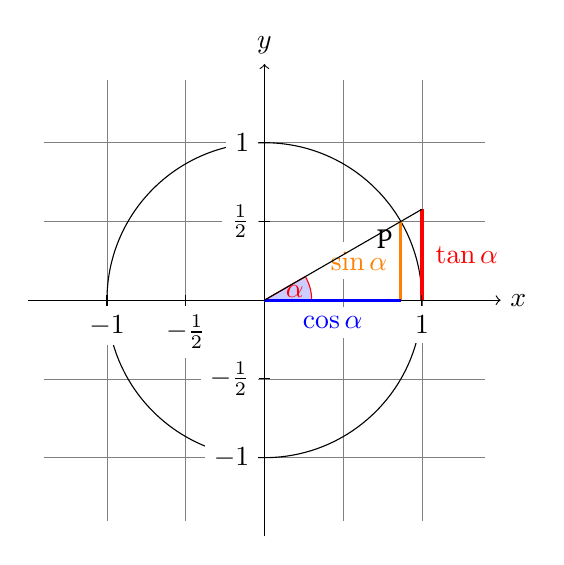
\begin{tikzpicture}[scale=2]
			\draw[step=.5cm,gray,very thin] (-1.4,-1.4) grid (1.4,1.4);
			\filldraw[fill=blue!20,draw=red] (0,0) -- (3mm,0mm)
				arc [start angle=0, end angle=30, radius=3mm] -- cycle;
			\node[red] at (15:2mm) {$\alpha$};
			\draw[->] (-1.5,0) -- (1.5,0) coordinate (x axis)node[right]{$x$};
			\draw[->] (0,-1.5) -- (0,1.5) coordinate (y axis)node[above]{$y$};
			\draw (0,0) circle [radius=1cm];
			\draw[very thick,orange]
				(30:1cm) -- node[left=1pt,fill=white] {$\sin \alpha$} (30:1cm |- x axis);
			\draw[very thick,blue]
				(30:1cm |- x axis) -- node[below=2pt,fill=white] {$\cos \alpha$} (0,0);
			\path [name path=upward line] (1,0) -- (1,1);
			\path [name path=sloped line] (0,0) -- (30:1.5cm);
			\draw [name intersections={of=upward line and sloped line, by=t}]
				[very thick,red] (1,0) -- node [right=1pt,fill=white]
				{$\displaystyle \tan \alpha$} (t);
			\draw (0,0) -- (t);
			\node[anchor=north east,inner sep=1mm] at (30:1cm){P};
			\foreach \x/\xtext in {-1, -0.5/-\frac{1}{2}, 1}
			\draw (\x cm,1pt) -- (\x cm,-1pt) node[anchor=north,fill=white] {$\xtext$};
			\foreach \y/\ytext in {-1, -0.5/-\frac{1}{2}, 0.5/\frac{1}{2}, 1}
			\draw (1pt,\y cm) -- (-1pt,\y cm) node[anchor=east,fill=white] {$\ytext$};
		\end{tikzpicture}
	\end{wrapfigure}
	We define $\sin \alpha$ and $\cos \alpha$ to be the the y-coordinate and x-coordinate of $P$ respectively (and ignore $\tan \alpha$ for now). We can observe serveral interesting properties of this definition regarding the sign of the trigonometric functions.
	\begin{enumerate}
		\item For $0 < \alpha < 90^o$, the values for $\sin \alpha, \cos \alpha$ are exactly the \textbf{same (including the sign)} as our previous definitions because the radius of the circle is $1$.
		\item For $90^o < \alpha < 180^o$, the values for $\cos \alpha$ becomes negative, while $\sin \alpha$ remains positive.
		\item For $180^o < \alpha < 270^o$, both the values for $\sin \alpha$ and $\cos \alpha$ become negative.
		\item For $270^o < \alpha < 360^o$, the value for $\sin \alpha$ is negative and the value for $\cos \alpha$ is positive.
		\item For $\alpha > 360^o$, what will happen?
		\item For $\alpha < 0^o$, what will happen?
	\end{enumerate}
}


{
	\begin{wrapfigure}[]{l}{0pt}
		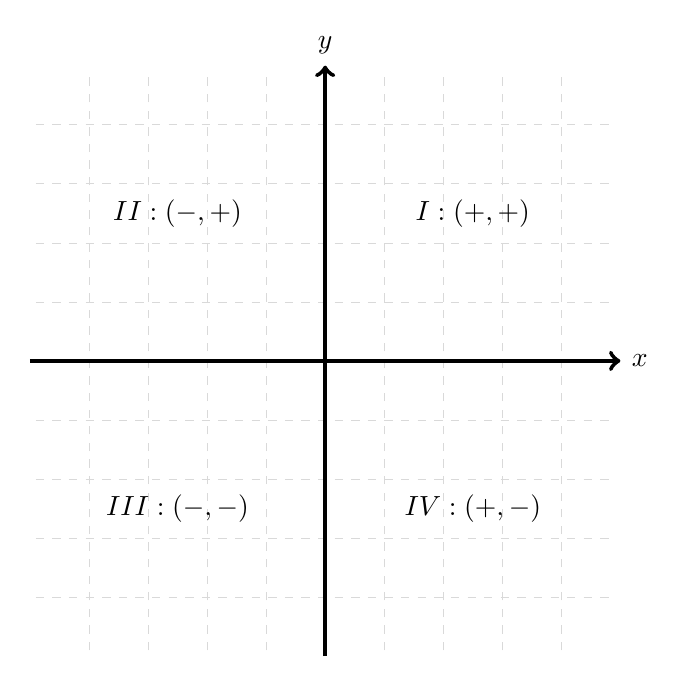
\begin{tikzpicture}[scale=0.75]
			\draw[help lines, color=gray!30, dashed] (-4.9,-4.9) grid (4.9,4.9);
			\draw[->,ultra thick] (-5,0)--(5,0) node[right]{$x$};
			\draw[->,ultra thick] (0,-5)--(0,5) node[above]{$y$};
			\node at (2.5, 2.5){$I: (+,+)$};
			\node at (-2.5, 2.5){$II: (-,+)$};
			\node at (-2.5, -2.5){$III: (-,-)$};
			\node at (2.5, -2.5){$IV: (+,-)$};
		\end{tikzpicture}
	\end{wrapfigure}

	Do we need to remember these facts? No, because it's just about the signs of x-coordinate and y-coordinate in different quadrants. 

	$\sin \alpha$ is only concerned with y-coordinate, so we can look at the sign of y-coordinate. In other words, it is positive in the I and II quadrant and negative in the III and IV quadrant.
	This means that $\sin \alpha$ is positive if $0^o < \alpha < 180^o$. and negative if $180^o < \alpha < 360^o$

	$\cos \alpha$ is only concerned with x-coordinate, so we can look at the sign of x-coordinate. In other words, it is positive in the I and IV quadrant and negative in the II and III quadrant. This means that $\cos \alpha$ is positive if $0^o < \alpha < 90^o$ or $270^o < \alpha < 360^o$ and negative if $90^o < 270^o$.

	For $\tan \alpha = \frac{\sin \alpha}{\cos \alpha}$, as we already know the sign of $\sin \alpha$ and $\cos \alpha$ in all quadrants, we also know the sign of $\tan \alpha$. $\tan \alpha$ is positive in \emph{I/II/III/IV (circle options that apply)} quadrant and negative in \emph{I/II/III/IV (circle options that apply)} quadrant. This means that $\tan \alpha$ is positive when \rule{6cm}{0.15mm} and negative when \rule{6cm}{0.15mm}

	Now check your result against the line marked $\tan \alpha$. First, do you see why the signed length of the line denotes the value of $\tan \alpha$? Second, does the sign of it match what you write?
}


\section{Values of trigonometric functions}
{
\begin{wrapfigure}{r}{0pt}
	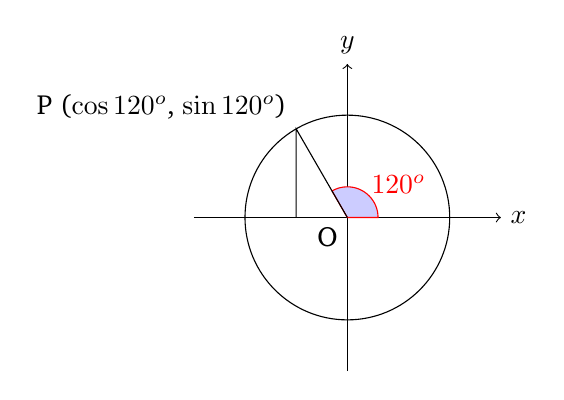
\begin{tikzpicture}[scale=1.3]
		\draw[->] (-1.5,0) -- (1.5,0) coordinate (x axis)node[right]{$x$};
		\draw[->] (0,-1.5) -- (0,1.5) coordinate (y axis)node[above]{$y$};
		\draw[color=black] (0,0) circle (1);
		\filldraw[fill=blue!20,draw=red] (0,0) -- (3mm,0mm)
			arc [start angle=0, end angle=120, radius=3mm] -- cycle;
		\node[anchor=north east] at (0,0) {O};
		\node[red, anchor=south west, inner sep=3mm] at (0,0) {$120^o$};
		\draw (0,0) -- (120:1)  node[anchor=south east]{P ($\cos 120^o$, $\sin 120^o$)} -- (180:{-cos(120)});
	\end{tikzpicture}
\end{wrapfigure}
Then we move on to find the value of $\sin \alpha$ where $\alpha = 120^o$ as an example. We draw a line with length 1 making an angle of $120^o$ with the positive x-axis like so:

The coordinate of $P$ is $(\cos 120^o, \sin 120^o)$ by definition. We can find the value of it by considering the right angled triangle in the II quadrant.
}
Since the radius of the circle is $1$ and the angle that $OP$ makes with the negative x-axis is $60^o$. We find that $\cos 120^o = -\cos 60^o$ and $\sin 120^o = \sin 60^o$

\begin{figure}[H]
	\centering
	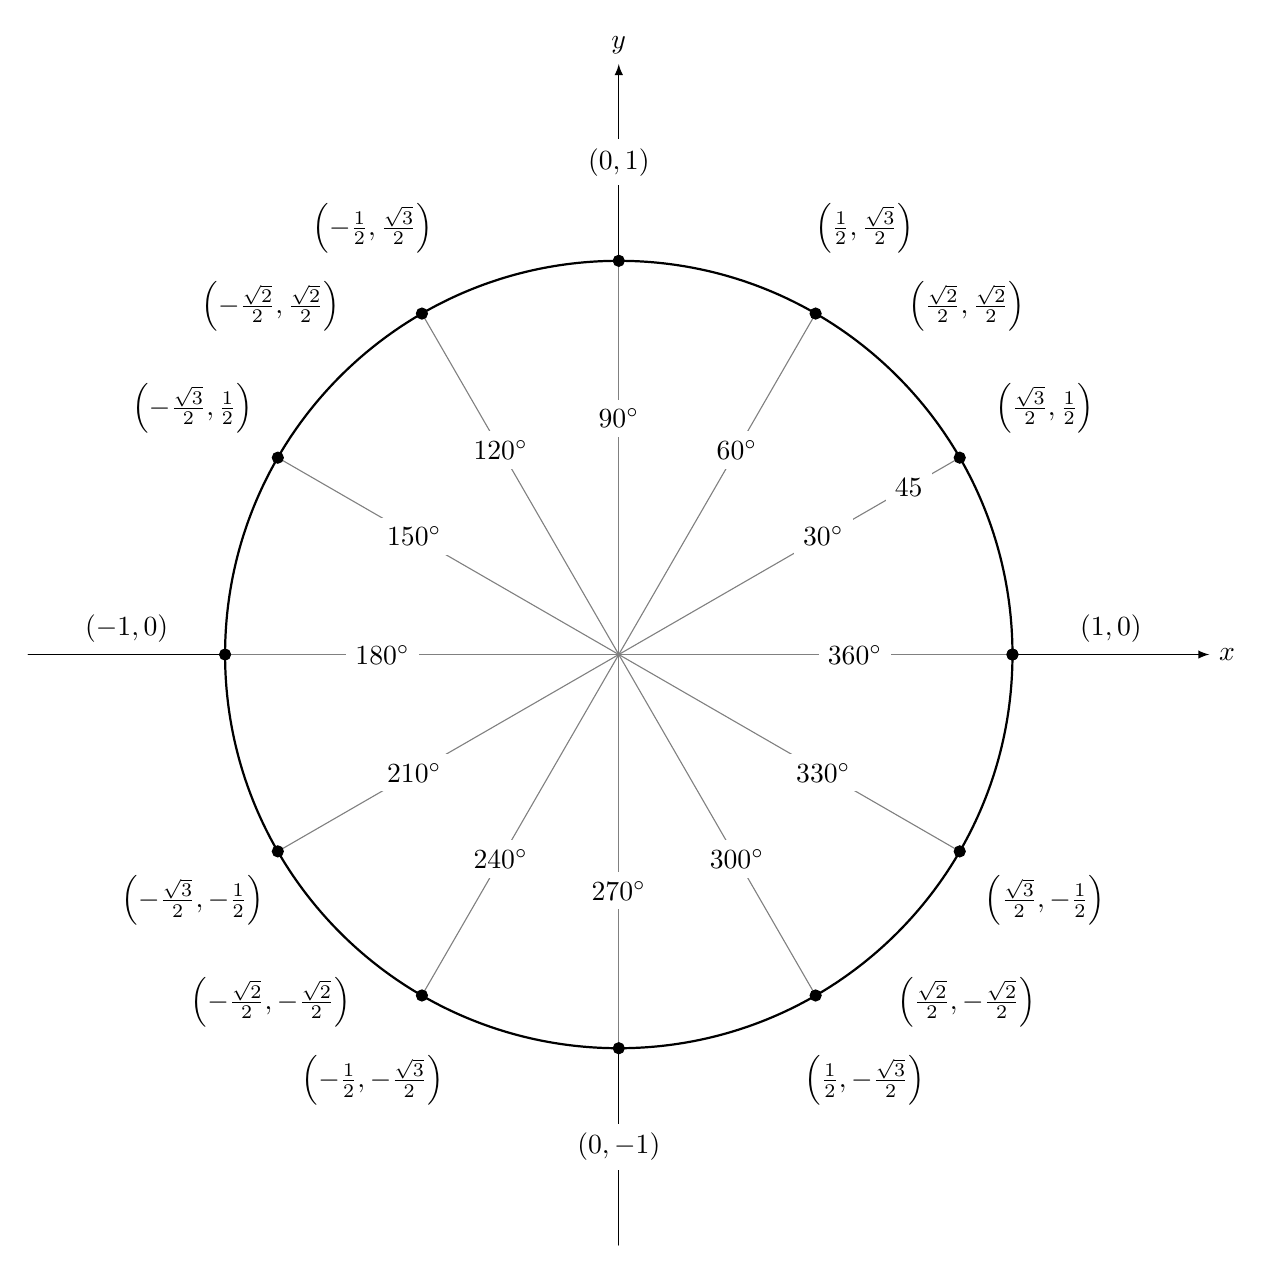
\begin{tikzpicture}[scale=5,cap=round,>=latex]
		% draw the coordinates
		\draw[->] (-1.5cm,0cm) -- (1.5cm,0cm) node[right,fill=white] {$x$};
		\draw[->] (0cm,-1.5cm) -- (0cm,1.5cm) node[above,fill=white] {$y$};

		% draw the unit circle
		\draw[thick] (0cm,0cm) circle(1cm);

		\foreach \x in {0,30,...,360} {
			% lines from center to point
			\draw[gray] (0cm,0cm) -- (\x:1cm);
			% dots at each point
			\filldraw[black] (\x:1cm) circle(0.4pt);
			% draw each angle in degrees
			\draw (\x:0.6cm) node[fill=white] {$\x^\circ$};
		}

		% draw each angle in radians
		\foreach \x/\xtext in {
			30/
			45/
			60/
			90/
			120/
			135/
			150/
			180/
			210/
			225/
			240/
			270/
			300/
			315/
			330/
		360/}
		\draw (\x:0.85cm) node[fill=white] {$\xtext$};

		\foreach \x/\xtext/\y in {
			% the coordinates for the first quadrant
			30/\frac{\sqrt{3}}{2}/\frac{1}{2},
			45/\frac{\sqrt{2}}{2}/\frac{\sqrt{2}}{2},
			60/\frac{1}{2}/\frac{\sqrt{3}}{2},
			% the coordinates for the second quadrant
			150/-\frac{\sqrt{3}}{2}/\frac{1}{2},
			135/-\frac{\sqrt{2}}{2}/\frac{\sqrt{2}}{2},
			120/-\frac{1}{2}/\frac{\sqrt{3}}{2},
			% the coordinates for the third quadrant
			210/-\frac{\sqrt{3}}{2}/-\frac{1}{2},
			225/-\frac{\sqrt{2}}{2}/-\frac{\sqrt{2}}{2},
			240/-\frac{1}{2}/-\frac{\sqrt{3}}{2},
			% the coordinates for the fourth quadrant
			330/\frac{\sqrt{3}}{2}/-\frac{1}{2},
			315/\frac{\sqrt{2}}{2}/-\frac{\sqrt{2}}{2},
		300/\frac{1}{2}/-\frac{\sqrt{3}}{2}}
		\draw (\x:1.25cm) node[fill=white] {$\left(\xtext,\y\right)$};

		% draw the horizontal and vertical coordinates
		% the placement is better this way
		\draw (-1.25cm,0cm) node[above=1pt] {$(-1,0)$}
			(1.25cm,0cm)  node[above=1pt] {$(1,0)$}
			(0cm,-1.25cm) node[fill=white] {$(0,-1)$}
			(0cm,1.25cm)  node[fill=white] {$(0,1)$};
	\end{tikzpicture}
\end{figure}
Based on the given coordinates, let's try to find the following values.
\begin{problemslist}
\item Find the values of $\sin 60^o$, $\cos 60^o$ and $\tan 60^o$.
\item Find the values of $\sin 120^o$, $\cos 120^o$ and $\tan 120^o$.
\item Find the values of $\sin 240^o$, $\cos 240^o$ and $\tan 240^o$.
\item Find the values of $\sin 390^o$, $\cos 390^o$ and $\tan 390^o$.
\item Find the values of $\sin 600^o$, $\cos 600^o$ and $\tan 600^o$.
\item Find the values of $\sin -30^o$, $\cos -30^o$ and $\tan -30^o$.
\item Find the values of $\sin 180^o$, $\cos 180^o$ and $\tan 180^o$.
\item Find the values of $\sin 90^o$, $\cos 90^o$ and $\tan 90^o$.
\end{problemslist}

We now consider more arbitary angles.

\begin{problemslist}
\item Given that $\sin 49^o = 0.754$ correct to 3 significant figures, find the values of $\sin 229^o$, $\cos 229^o$ and $\tan 229^o$.
\item Given that $\sin 29^o = 0.485$ correct to 3 significant figures, find the values of $\sin (-29^o)$, $\cos (-29^o)$ and $\tan (-29^o)$. Verify the two trigonometric identities that you learnt in the past holds for : $\tan(-29^o) = \frac{\sin(-29^o)}{\cos(-29^o)}$ and $\sin^2(-29^o) + \cos^2(-29^o) = 1$
\end{problemslist}

\section{Problems of type $\sin(90^o/180^o/270^o \pm \theta)$}
To kick off this chapter, let me present to you one identity that may seem shocking at first: \[\sin(\theta+90) = \cos(\theta)\]

To see why this is true, we only consider $0 < \theta < 90^o$ first. Then $\theta + 90^o$ lies in the II quadrant.

{
\begin{wrapfigure}{r}{0pt}
	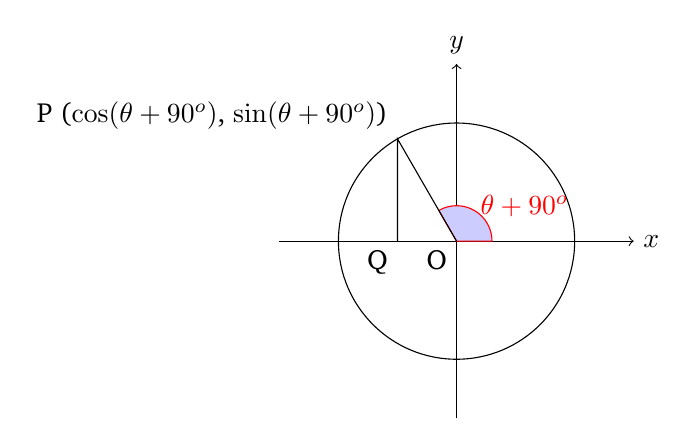
\begin{tikzpicture}[scale=1.5]
		\draw[->] (-1.5,0) -- (1.5,0) coordinate (x axis)node[right]{$x$};
		\draw[->] (0,-1.5) -- (0,1.5) coordinate (y axis)node[above]{$y$};
		\draw[color=black] (0,0) circle (1);
		\filldraw[fill=blue!20,draw=red] (0,0) -- (3mm,0mm)
			arc [start angle=0, end angle=120, radius=3mm] -- cycle;
		\node[anchor=north east] at (0,0) {O};
		\node[red, anchor=south west, inner sep=3mm] at (0,0) {$\theta + 90^o$};
		\draw node(O){}(0,0) -- (120:1)  node[anchor=south east](P){P ($\cos (\theta + 90^o)$, $\sin (\theta + 90^o)$)} -- (180:{-cos(120)}) node[anchor=north east](Q){Q};
	\end{tikzpicture}
\end{wrapfigure}

By doing some angle chasing, we find that $\angle OPQ = \theta$ and hence the $OQ = \sin \theta$, which means the y-coordinate of $P = \sin (\theta + 90^o)$ is actually just $\cos \theta$ in disguise. Note that we have discussed in previous sections that $\sin (\theta + 90^o)$ will be positive since $\theta + 90^o$ is in the II quadrant.

Although this derivation only proves that the identity is true for $0^o < \theta < 90^o$, \textbf{the identity is actually true for all $\theta$}. This is because of the symmetry that lies in trigonometric functions. Hence, when we treat expression of the form $\sin(90^o/180^o/270^o \pm \theta)$ and we want to simplify it, we can always $\textbf{assume $\theta$ is in the I quadrant}$ and derive a simplier expression from the original one.

If we consider the x-coordinate of $P$ instead, you will see that since OQ = $\sin \theta$ and and $\cos(\theta + 90^o)$ lies in the negative x-axis, we get another identity $\cos(\theta+90^o) = -\sin \theta$.
}

\begin{problemslist}
\item Simplify $\sin(\theta+180^o)$, $\cos(\theta+180^o)$ and $\tan(\theta+180^o)$.
\item Simplify $\sin(\theta+270^o)$, $\cos(\theta+270^o)$ and $\tan(\theta+270^o)$.
\item Simplify $\sin(\theta-90^o)$, $\cos(\theta-90^o)$ and $\tan(\theta-90^o)$.
\item Simplify $\sin(\theta-90^o)$, $\cos(\theta-90^o)$ and $\tan(\theta-90^o)$.
\item Simplify $\frac{\sin(270^o - \theta)}{\cos(180^o-\theta)}$
\item Simplify $\tan(270^o+\theta) \cos(180^o+\theta)$
\item Simplify $\frac{2-2\cos^2(270^o-\theta)}{\sin(180^o+\theta)\tan(270^o-\theta)}$
\item Find the value of $\cos 1^o + \cos 2^o + ... + \cos 179^o$
\item Find the value of $\tan 91^o \cdot \tan 179^o + \tan 92^o \cdot 178^o + \tan 93^o \cdot 177^o + ... + \tan 179^o \cdot \tan 91^o$
\item Given that $\cos (270^o + \theta) = -0.6$ and $\cos \theta > 0$, find the values of $\sin \theta, \cos \theta$ and $\tan \theta$.
\item Given that $\tan (180^o - \theta) = 3$, find the values of $\sin \theta, \cos \theta$ and $\tan \theta$
\item Given that $\cos (360^o - \theta) = \frac{2}{5}$, find the value of $\frac{4 \sin 210^o \cdot \cos (-\theta)}{1 + \tan^2(180^o + \theta)}$
\item $\alpha, \beta$ and $\theta$ are the interior angles of a triangle with $\alpha + \beta = 90^o$. Prove the following identities:

	(a) $\sin \alpha - \cos \beta = \cos \theta$

	(b) $\tan \alpha \tan \beta - \tan (\theta){2} = 0$

	(c) $\sin \alpha = \sin \beta \tan (\theta - \beta)$

	(d) $\cos^2 \alpha + \cos^2 \beta + \cos 2\theta = 0$

\end{problemslist}

\section{Solving trigonometric equations}

Example:
If $\sin x = -0.6$, find $x$ where $0 \leq x \leq 360^o$.

Solution:
To approach this type of problem, we first need to find out which quadrant does $x$ lie in. In this case, only quadrant III and IV are possible since $\sin x$ is negative. Then we can draw the circle that we've already been very familiar with to find the value of $x$.

\begin{wrapfigure}{r}{0pt}
	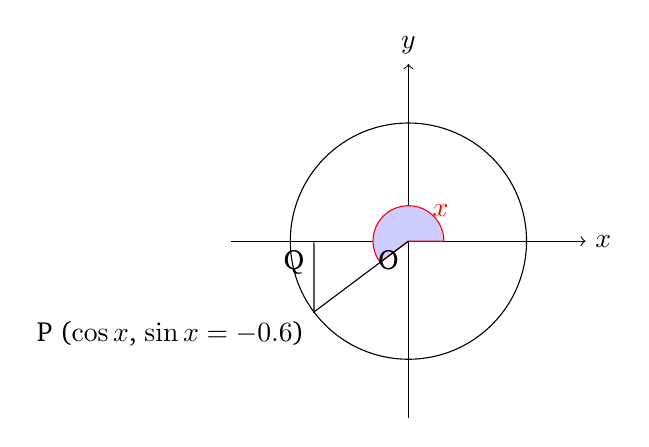
\begin{tikzpicture}[scale=1.5]
		\draw[->] (-1.5,0) -- (1.5,0) coordinate (x axis)node[right]{$x$};
		\draw[->] (0,-1.5) -- (0,1.5) coordinate (y axis)node[above]{$y$};
		\draw[color=black] (0,0) circle (1);
		\filldraw[fill=blue!20,draw=red] (0,0) -- (3mm,0mm)
			arc [start angle=0, end angle=216.869, radius=3mm] -- cycle;
		\node[anchor=north east] at (0,0) {O};
		\node[red, anchor=south west, inner sep=3mm] at (0,0) {$x$};
		\draw node(O){}(0,0) -- (216.869:1)  node[anchor=north east](P){P ($\cos x$, $\sin x = -0.6$)} -- (-180:0.8) node[anchor=north east](Q){Q};
	\end{tikzpicture}
\end{wrapfigure}
We first deal with the angle in quadrant III, we consider the right-angled triangle OQP first (and ignore the signs first), we find that $\angle QOP = \sin^{-1}(0.6)$ and hence $x = 180^o + \angle QOP = 216.869^o$
Then we consider the angle in quadrant IV (not drawn in the figure) , by angle chasing you will be able to find that $\theta = 360^o - \sin^{-1}(0.6) = 323.1^o$

Many students may be tempted to try \\ 
$\sin^{-1}(-0.6)$. While the calculator can give you a correct $x$. This approach can only find 1 solution for $x$ when there may exist many (depending on the range of $x$ allowed). You will have to manually find the other solutions anyway.

\begin{problemslist}
\item If $\cos x=0.2$, find $x$, where $0^o \leq x \leq 360^o$.
\item Solve $4\cos x = 1$, where $0^o \leq x \leq 360^o$.
\item Solve $5\tan x = -3$, where $0^o \leq x \leq 360^o$.
\item Solve $\sqrt{3} \cos x = -1$, where $0^o < x < 180^o$.
\item Solve $-3\tan x = 7$, where $0^o \leq x < 360^o$.
\item Without using a calculator, find $\theta$ for each of the following, where $0^o < \theta < 360^o$

	(a) $\tan \theta = \tan 42^o$

	(b) $\cos \theta = -\cos 87^o$

	(c) $\sin \theta = \cos 1^o$

	(d) $\cos \theta = -\sin 63^o$

\end{problemslist}

\end{document}
